\chapter{Introduction} \label{chap:intro}


%###############################################################################################################################
%###############################################################################################################################
%###############################################################################################################################
\section{Nuclear Fusion}%
\label{sec:intro_whatisfusion}

\begin{figure}[t!]
    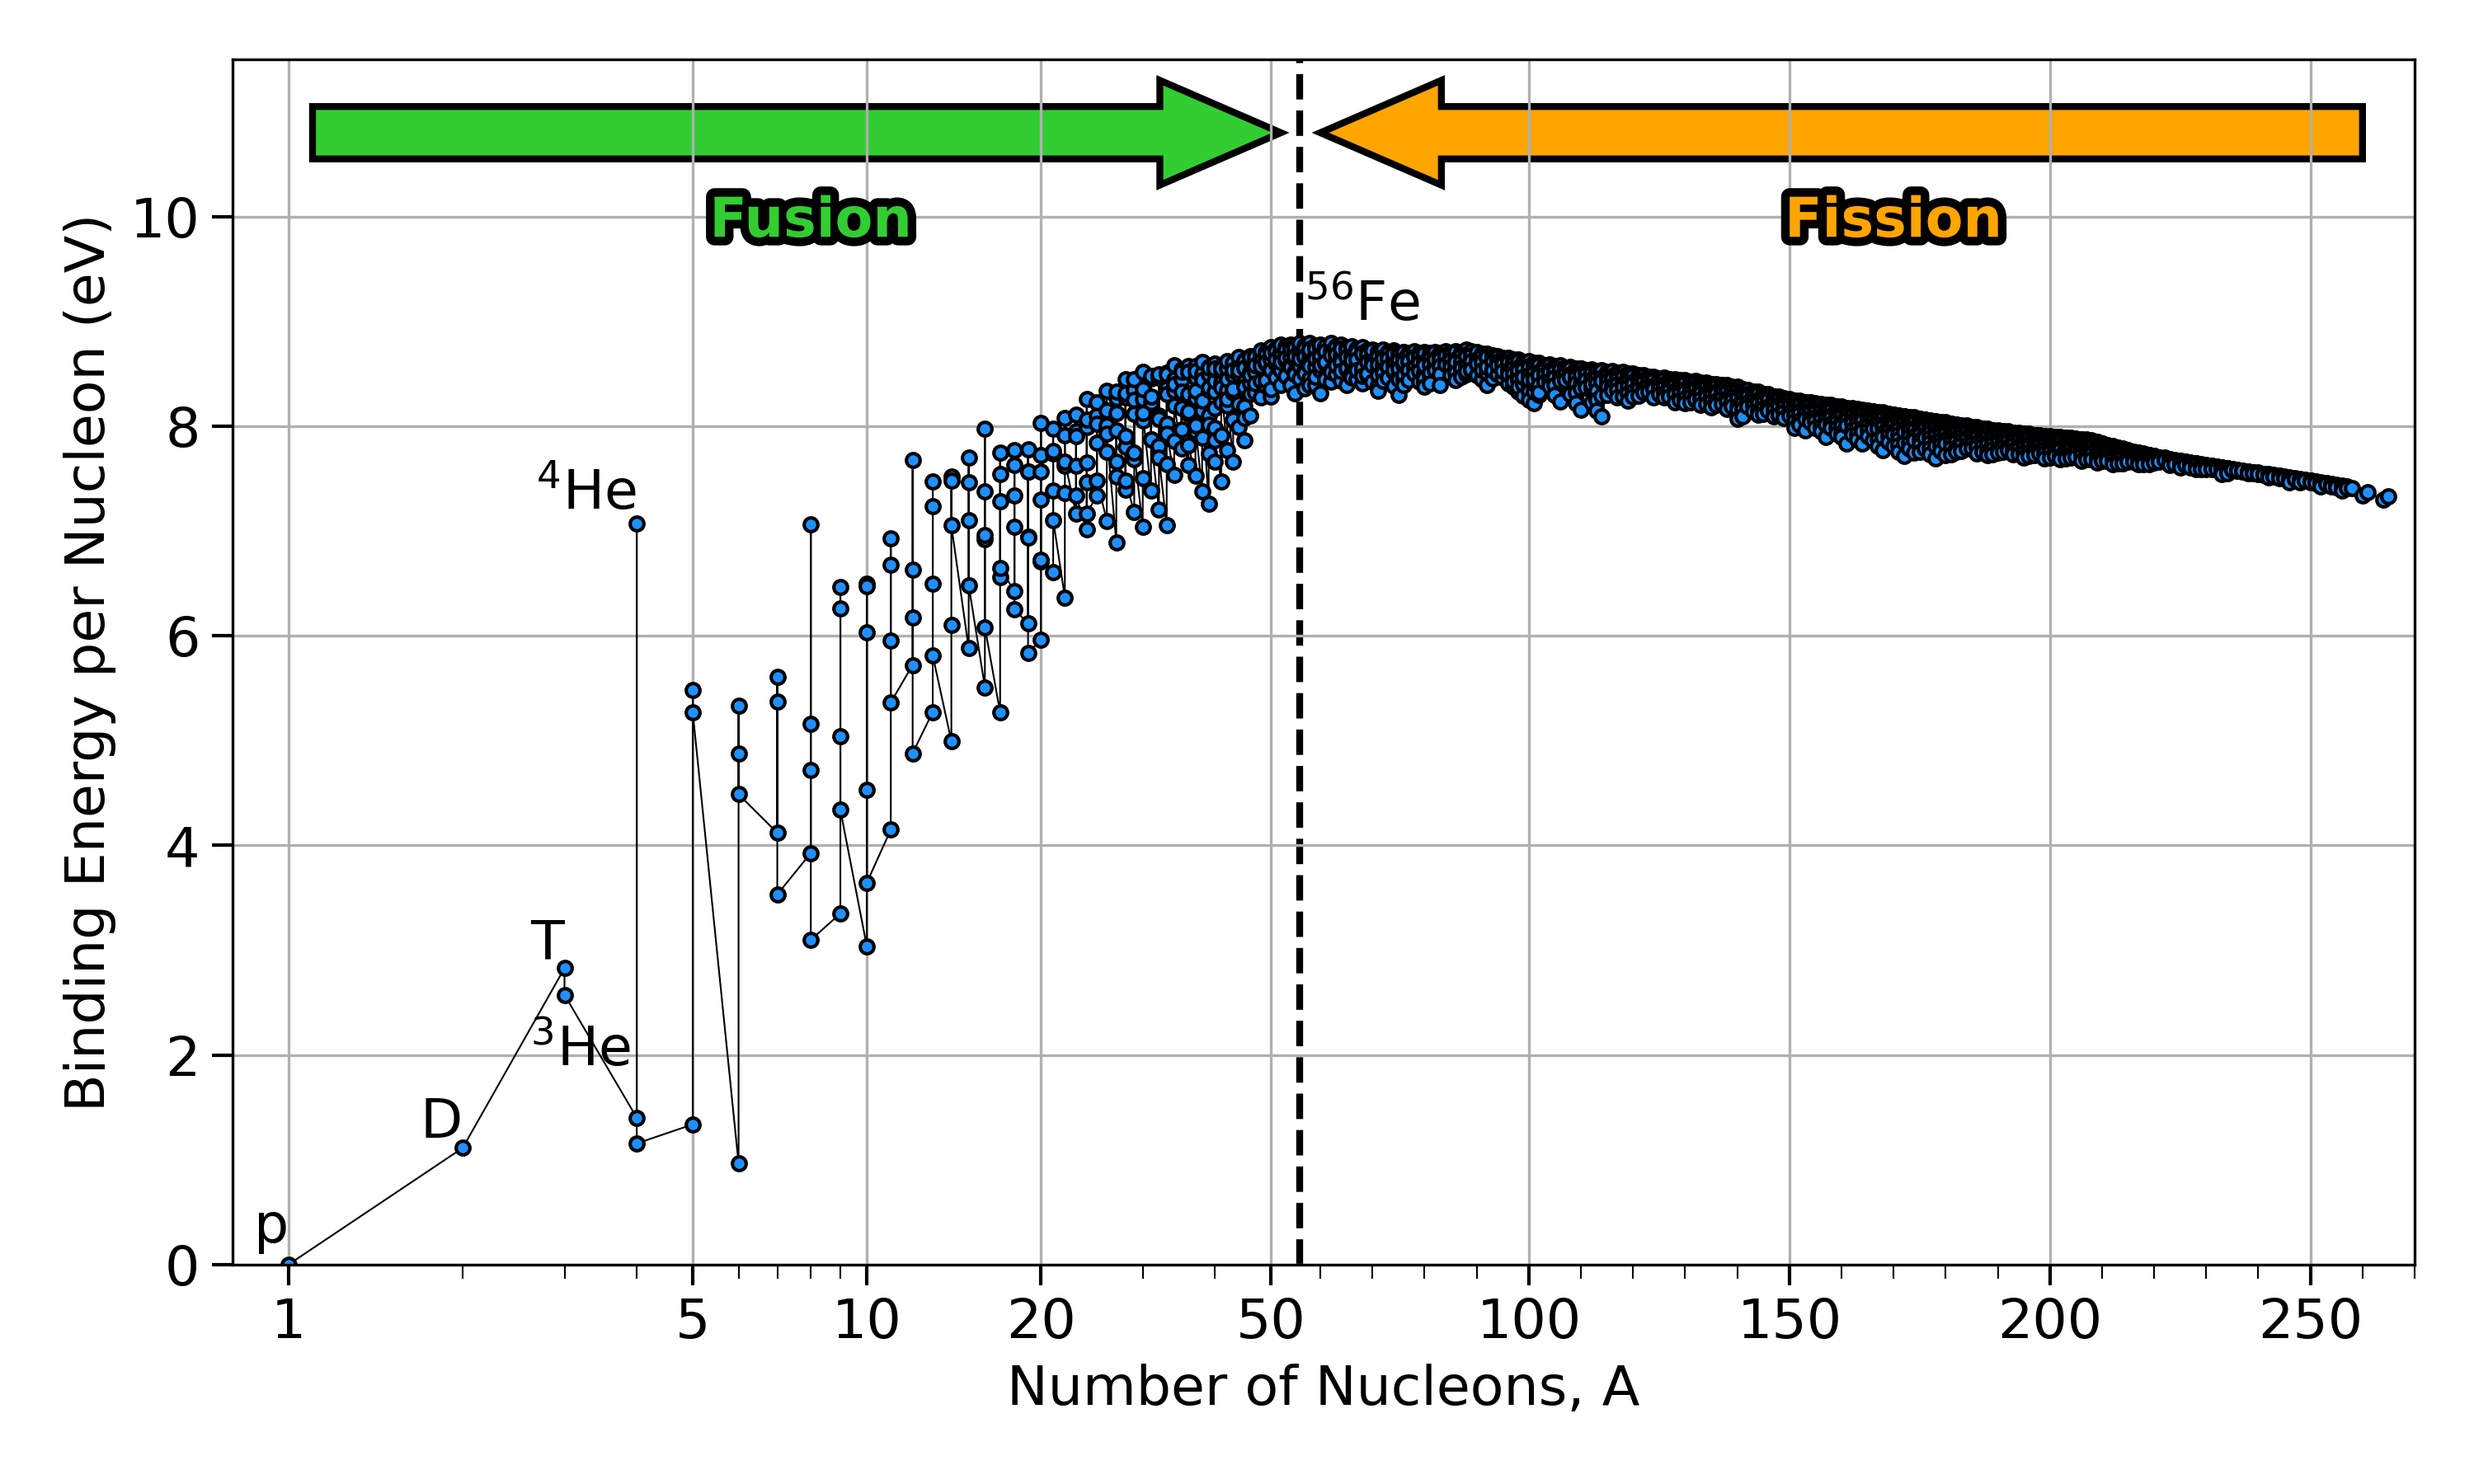
\includegraphics[width=0.9\linewidth]{Introduction/Images/BE_per_nucleon.png}
    \centering
    \caption{Binding energy per nucleon for common nuclear isotopes.
    Binding energy peaks close to iron, therefore energy is released for reactions which increase binding energy.
    ${}^{4}\text{He}$ has a particularly high binding energy and therefore fusion reactions which results in this isotope are strong candidates for fusion energy production.
    }%
    \label{fig:intro_BEperNucleon}
\end{figure}

Say what fusion is and compare to fission and other energy sources.
Give main reactions.

%###############################################################################################################################
%###############################################################################################################################
%###############################################################################################################################
\section{Inertial Confinement Fusion}%
\label{sec:intro_ICF}

Describe ICF vs MCF and MIF.

%################################################################################
%################################################################################
\subsection{Ignition Requirements}%
\label{sec:intro_icf_ignition}

Give Lawson and ICF version.

%################################################################################
%################################################################################
\subsection{Central Hotspot Ignition}%
\label{sec:intro_centralhotspot}

\begin{figure}[t!]
    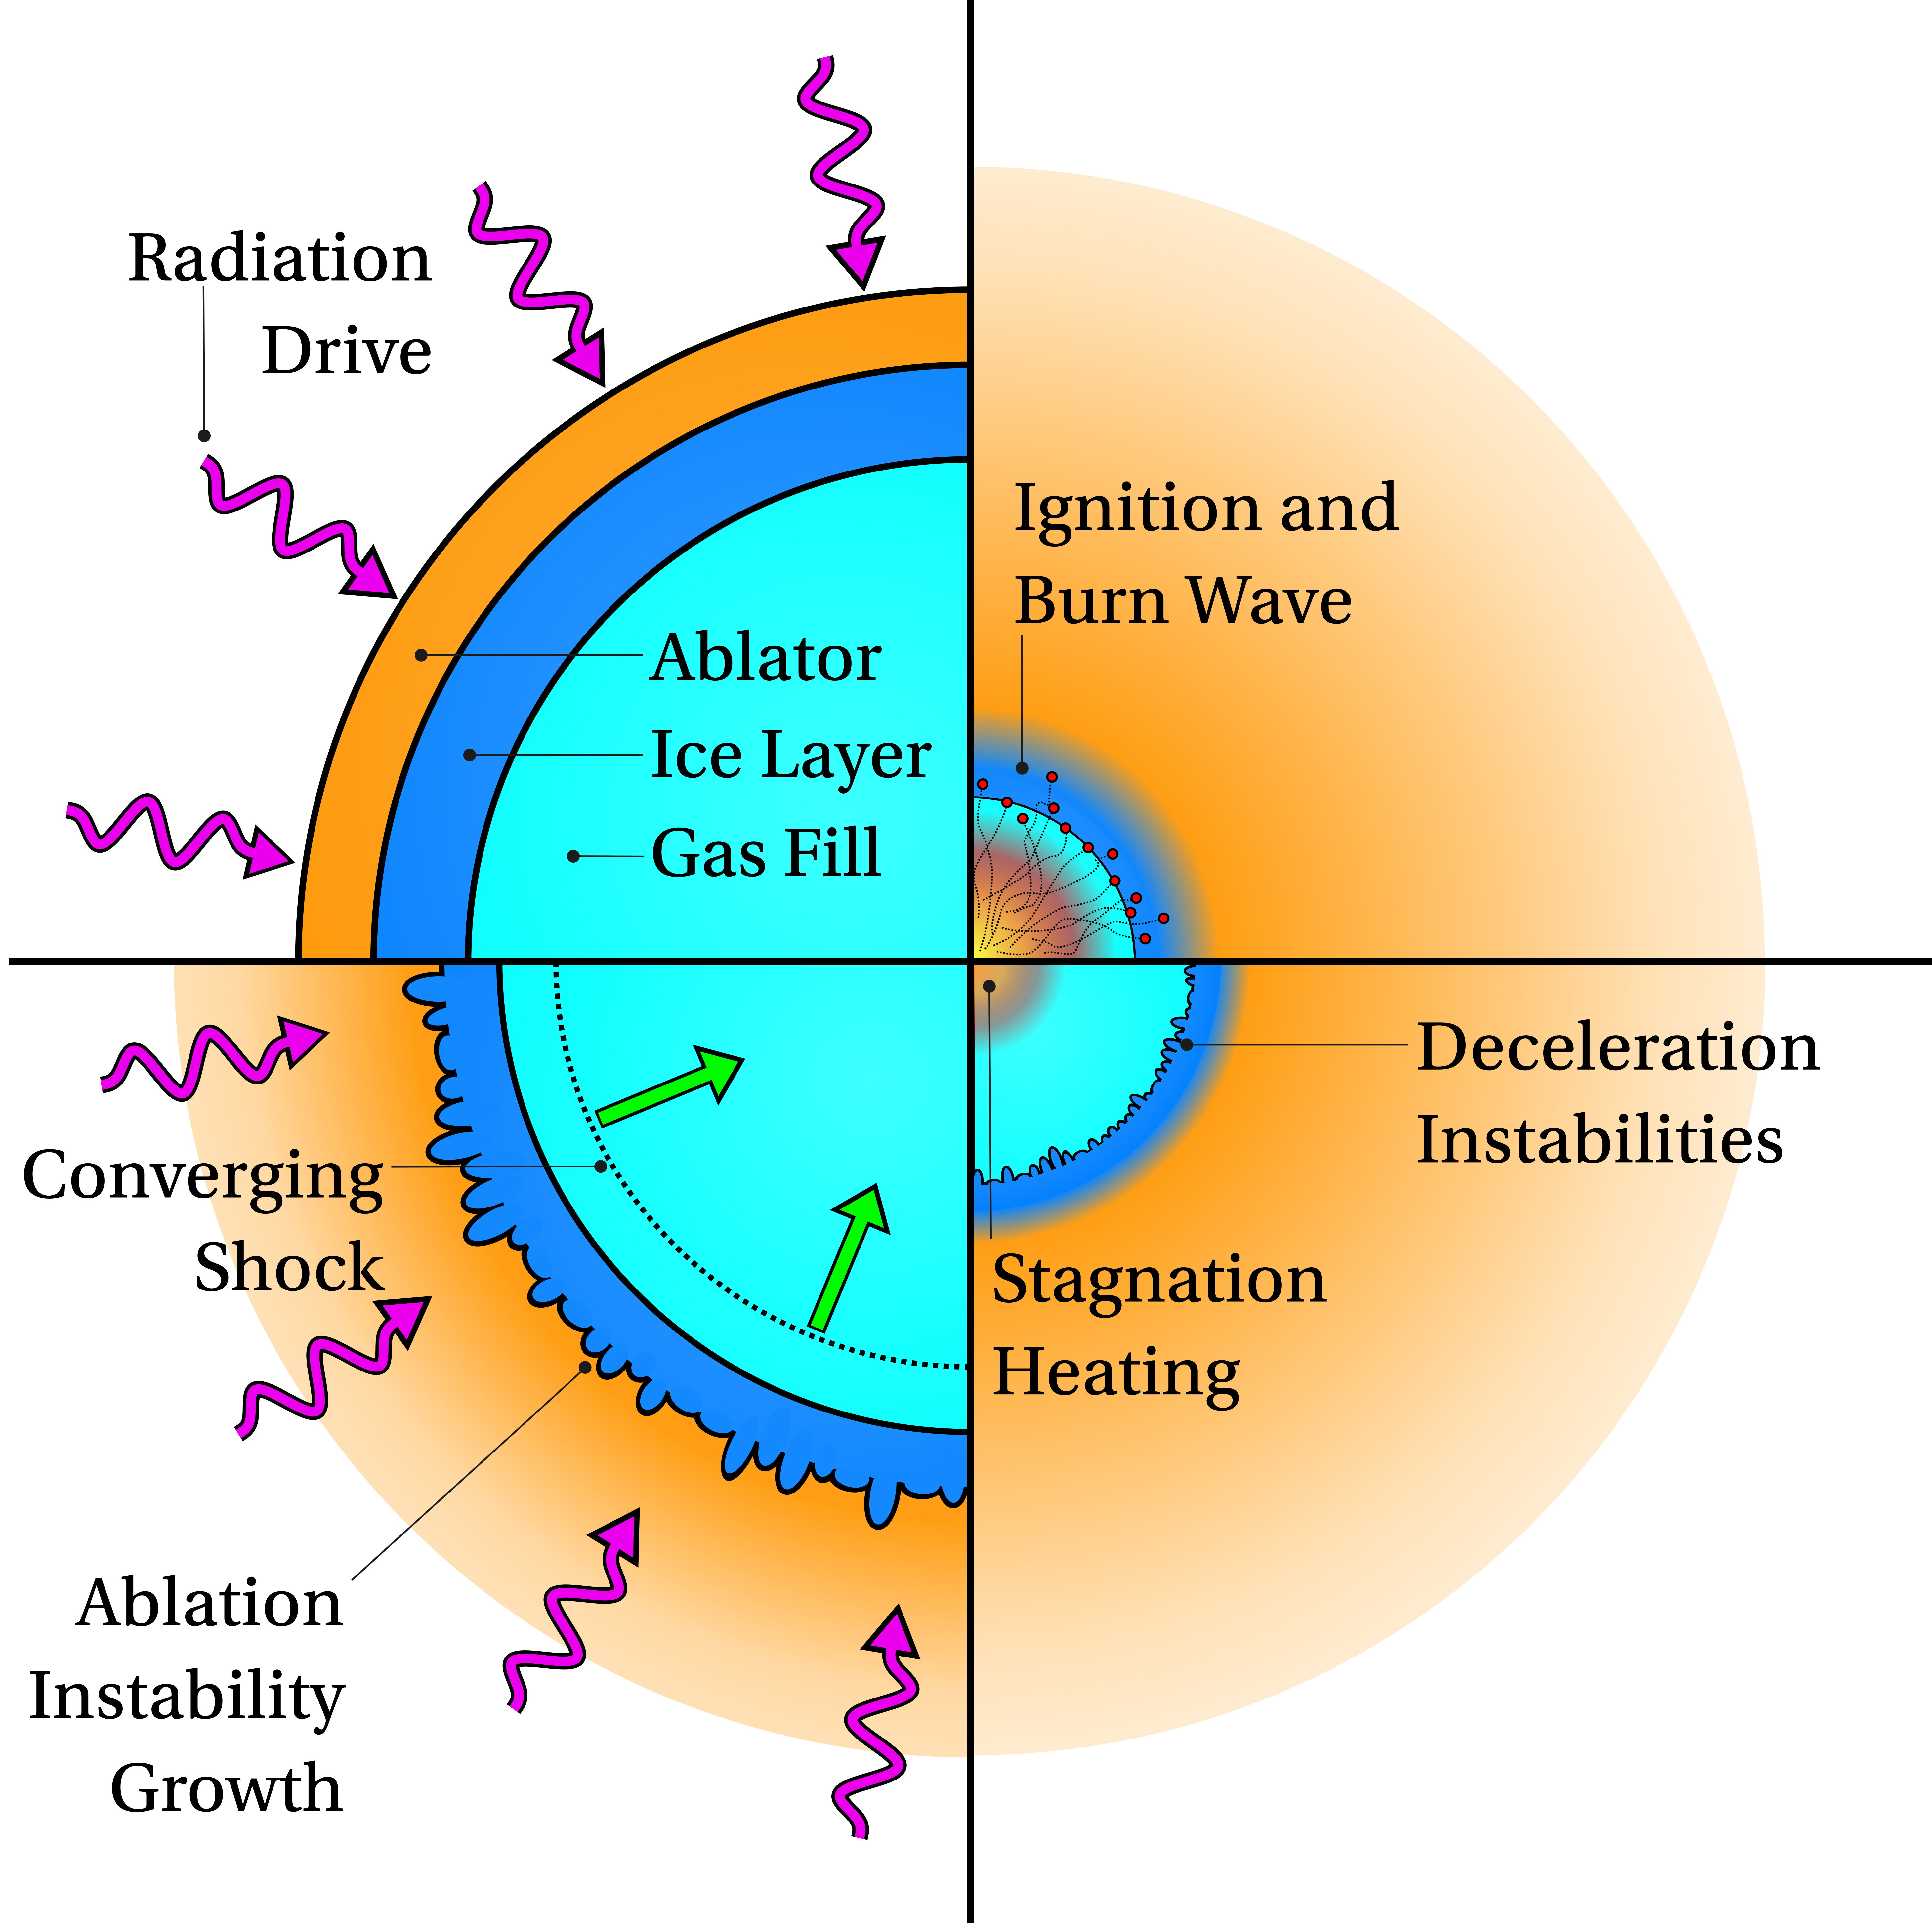
\includegraphics[width=0.7\linewidth]{Introduction/Images/hotspot ignition white.png}
    \centering
    \caption{Key Stages of the central hotspot ignition \ac{ICF} concept.
    }%
    \label{fig:intro_hotspot}
\end{figure}

Describe ablation pressure, ignite small volume of fuel etc.

%################################################################################
%################################################################################
\subsection{Alternative Approaches}%
\label{sec:intro_icf_alt}

Shock and fast ignition.

%###############################################################################################################################
%###############################################################################################################################
%###############################################################################################################################
\section{Current Experiments/ Main Approaches}%
\label{sec:intro_ICF}

Small intro on direct vs indirect.

%################################################################################
%################################################################################
\subsection{Indirect Drive}%
\label{sec:intro_indirect}

\begin{figure}[t!]
    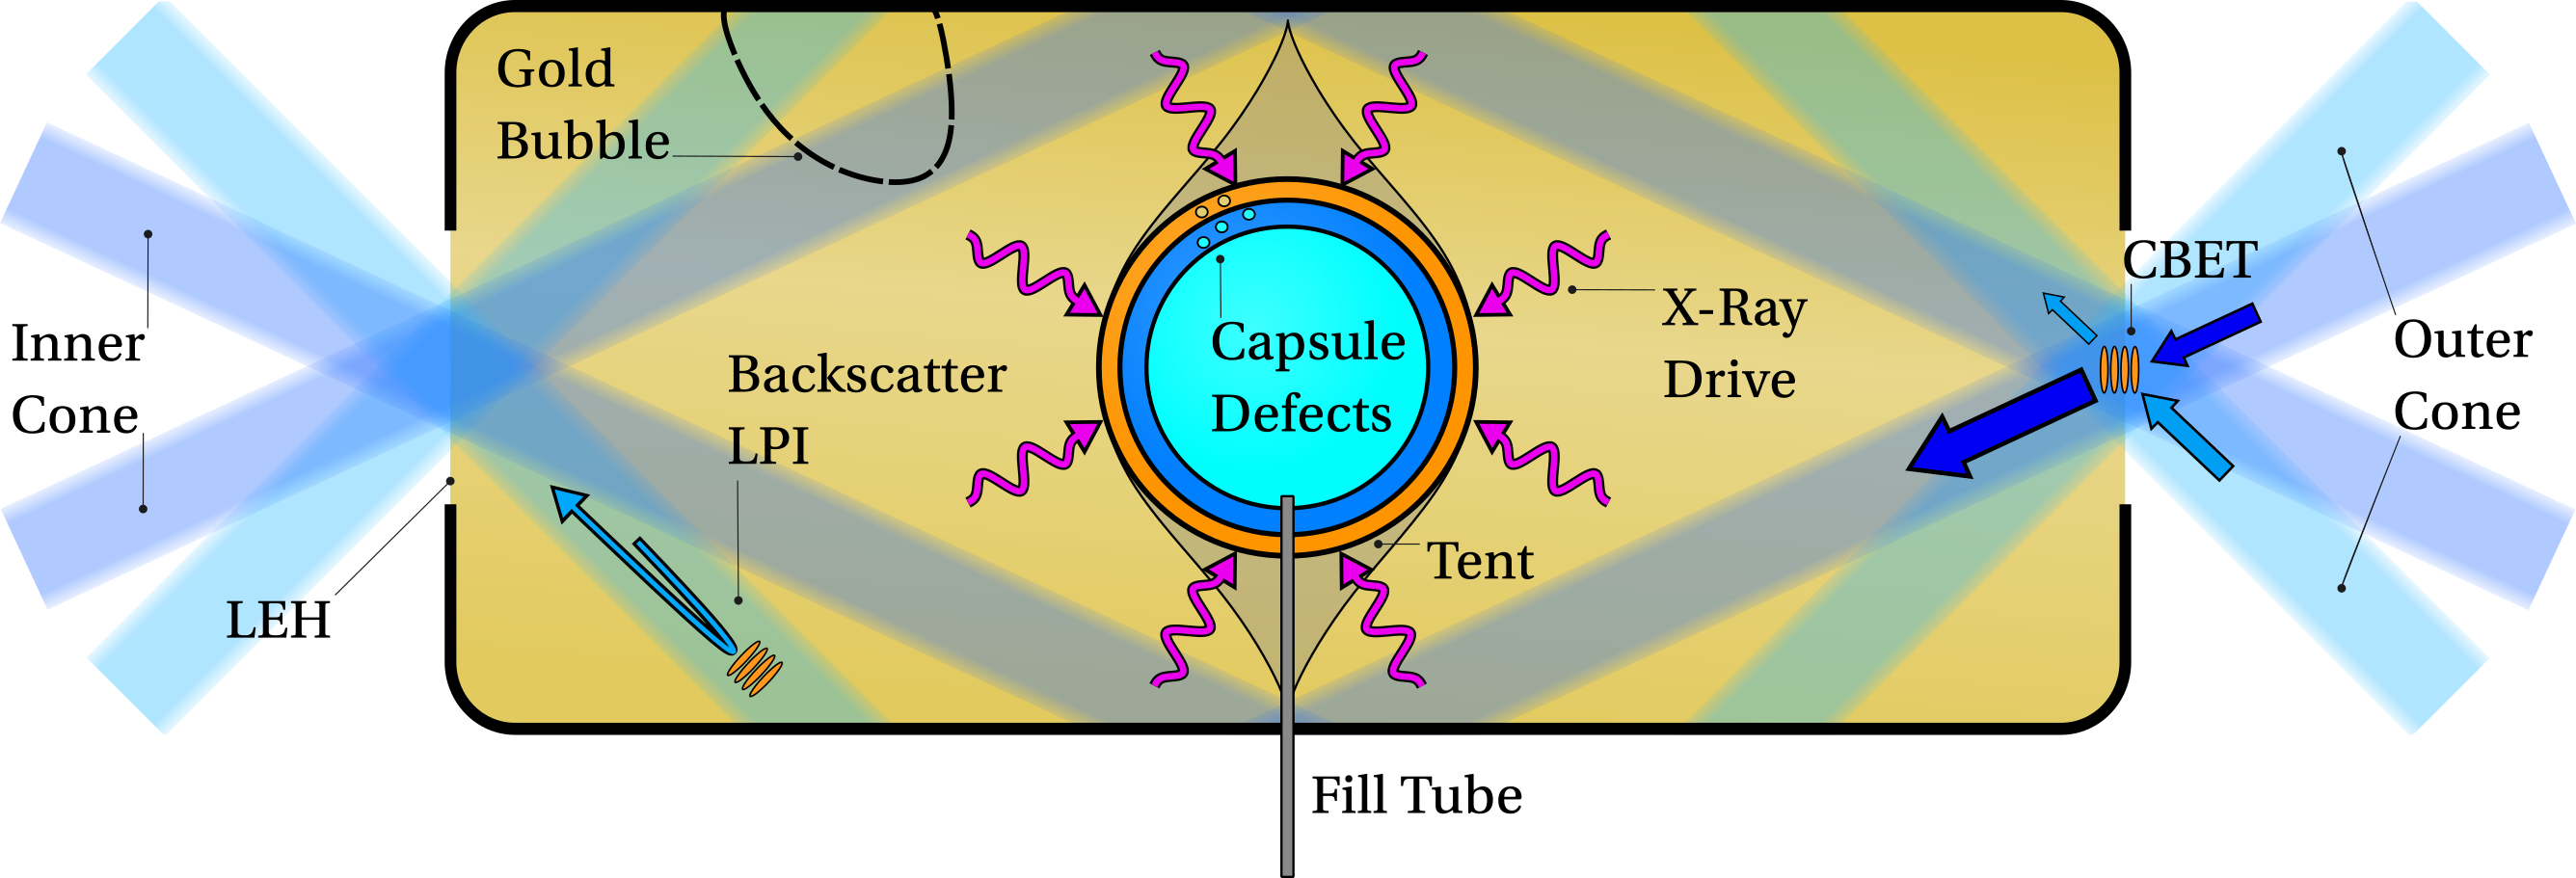
\includegraphics[width=\linewidth]{Introduction/Images/indirect icf white.png}
    \centering
    \caption{Schematic of the indirect-drive approach to \ac{ICF}.
    }%
    \label{fig:intro_indirect}
\end{figure}

Talk about all that jazz and give the diagram.
Talk about NIF and ignition, gain etc.

%################################################################################
%################################################################################
\subsection{Direct Drive}%
\label{sec:intro_direct}

\begin{figure}[t!]
    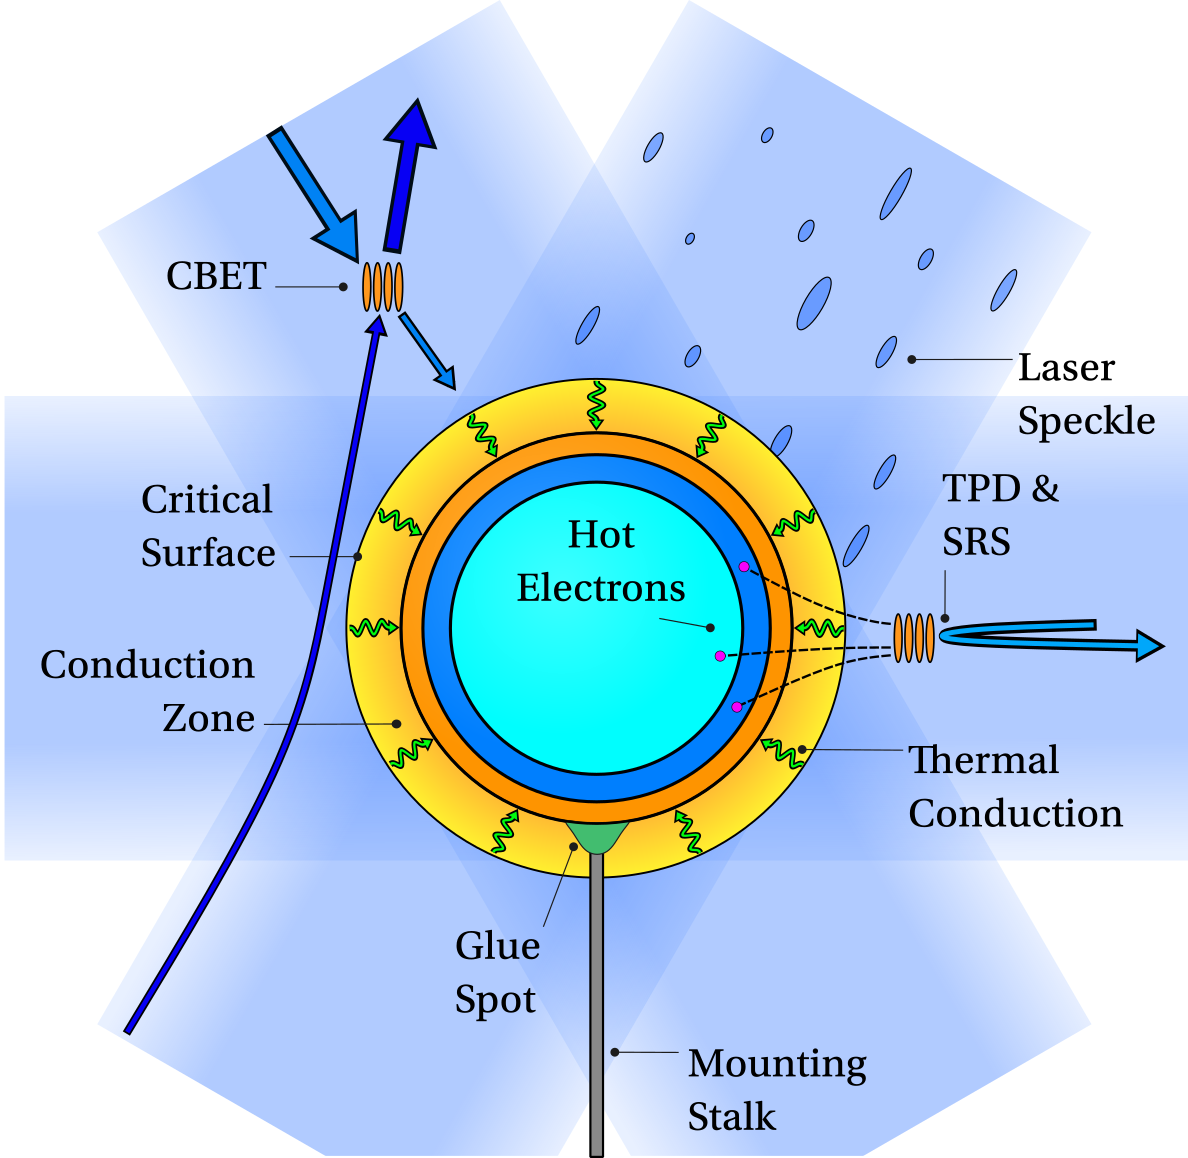
\includegraphics[width=0.7\linewidth]{Introduction/Images/direct icf white.png}
    \centering
    \caption{Schematic of the direct-drive approach to \ac{ICF}.
    }%
    \label{fig:intro_direct}
\end{figure}

Say its the assumed version for IFE.
Give a much more detailed anatomy of implosion, incl diagram.
Talk about hydro-scaled ignition etc.

%###############################################################################################################################
%###############################################################################################################################
%###############################################################################################################################
\section{Laser Interaction with Plasmas}%
\label{sec:intro_laserplasmas}

Understanding lasers is obviously crucial for Direct, indirect and hedp more generally.

%################################################################################
%################################################################################
\subsection{Regime of interest}%
\label{sec:intro_laser_regime}

Want collisional absorption and to avoid LPIs.
Therefore short wavelength, high power lasers, with limits to peak intensity.
Balance between $P_abl$ and high $I*lam^2$.

%################################################################################
%################################################################################
\subsection{ICF Relevant LPIs}%
\label{sec:intro_LPIs}

Damaging class of laser-plasma interactions for ICF.
Give diagram of how they work microphysically.
Include direct drive LPI diagram.
Introduce each in turn and say what they do for direct and indirect.

%###############################################################################################################################
%###############################################################################################################################
%###############################################################################################################################
\section{Objective of the work}%
\label{sec:intro_objective}

LPIs are important for current experiments.
Need to include models for them in integrated codes.
Also, next gen lasers will eliminate LPIs hopefully with bandwidth, so need to understand how they degrade current experiments to accurately extrapolate.
Create laser module for CHIMERA, specifically capable of modelling LPIs, and then see what their effect is for direct-drive.
